\documentclass[
  aps,
  prd,
  reprint,
  superscriptaddress,
  floatfix,
  amsmath,
  amssymb
]{revtex4-2}

\usepackage{xeCJK}
\setCJKmainfont{FandolSong-Regular.otf}[
  BoldFont=FandolHei-Regular.otf,
  ItalicFont=FandolKai-Regular.otf
]
\usepackage{booktabs}
\usepackage{graphicx}
\usepackage{hyperref}
\usepackage{xcolor}

\hypersetup{hidelinks}
\linespread{1.08}
\graphicspath{{figures/}}
\newcommand{\degc}{^\circ\mathrm{C}}
\newcommand{\tcell}[2][0.18\textwidth]{\begin{minipage}[t]{#1}\raggedright #2\end{minipage}}

\begin{document}

\title{温度对 CdZnTe/CdTe X 射线能量分辨探测器性能影响的文献综述\\
\large 面向 XRD/EDXRD、coherent scatter imaging 与相关能谱成像应用}
\author{刘禹泽}
\email{liuyuze23@mails.tsinghua.edu.cn}
\affiliation{清华大学工程物理系，北京 100084，中国}
\date{July 1, 2026}

\begin{abstract}
CdZnTe 和 CdTe 探测器常被视为 XRD、EDXRD、coherent scatter imaging、coded-aperture XRD、高通量光子计数和能谱成像中替代低温 Ge 探测器的关键高 $Z$ 半导体方案。本文基于已经精读和结构化提取的 21 篇本地文献，综述温度如何通过漏电流、电子噪声、能量分辨率、峰位漂移、极化、计数率能力和长期稳定性改变 CdZnTe/CdTe 能量分辨探测器的系统性能。核心结论是：CdZnTe，尤其 Redlen/eV Products high-flux CdZnTe，更适合室温或轻度控温下稳定工作，温控主要服务于 ASIC、基线、峰位和多模块标定；CdTe，尤其 Acrorad Schottky CdTe，更依赖低温、TEC/水冷、氮气或真空、防凝露和偏压刷新来延缓极化。降温通常降低漏电和噪声，但并不等于所有性能单调提升；最优温度应按目标通量、采集时间、能量分辨率、稳定性和工程代价共同确定。
\end{abstract}

\maketitle

\section{引言}

X 射线衍射成像、energy-dispersive X-ray diffraction (EDXRD)、coherent scatter imaging 和 coded-aperture XRD 的共同约束是：系统希望在有限采集时间内同时获得空间、能量和散射角信息，而探测器必须在吸收效率、能量分辨率、计数率、稳定性和可维护性之间折中。高纯 Ge 可以给出优异的能量分辨率，但深冷、真空和维护成本很难与安检、工业无损检测或便携式谱成像系统兼容。因此，CdZnTe 与 CdTe 因高 $Z$、宽禁带和近室温工作潜力，成为这些系统中反复出现的候选材料\cite{kosciesza2013,montemont2013,greenberg2014,greenberg2016,stryker2021}。

温度不是一个附属环境量。它决定热激发漏电流和接触注入电流，影响前端电子学噪声、阈值、基线漂移、陷阱退俘获、空间电荷、电场分布、极化速度和偏压后的历史效应。对 XRD/EDXRD 这类依赖峰位和谱形的应用，温度漂移最终会转化为材料识别误差、$q$ 分辨率劣化、标定失效或偏压刷新死时间。已有文献清楚显示，CdZnTe 与 CdTe 的温度响应并不等价：high-flux CdZnTe 常可在 $18$--$30\,\degc$ 轻度控温范围内稳定运行，而 Schottky CdTe 的极化时间常数和漏电流对 $0$--$30\,\degc$ 的变化极为敏感\cite{veale2020,cline2024,greiffenberg2025,astromskas2016,meyer2022}。

本文不把综述写成文献清单，而按证据图组织论证。图~\ref{fig:xdi} 和图~\ref{fig:coded} 给出 XRD/EDXRD 系统为什么需要温控而又不一定需要深冷；图~\ref{fig:redlen}--\ref{fig:cztpolar} 给出 CdZnTe 在近室温、轻度控温和高通量接触工程中的表现；图~\ref{fig:cdtemech}--\ref{fig:cdtestability} 给出 CdTe Schottky 温度、偏压历史和极化的直接证据。每组图注都明确区分晶体/样品温度、sensor temperature、模块/冷板温度、ASIC/板卡温度和环境温度，避免把不同文献中的 ``temperature'' 误合并为同一种物理量。

\begin{figure*}[t]
  \centering
  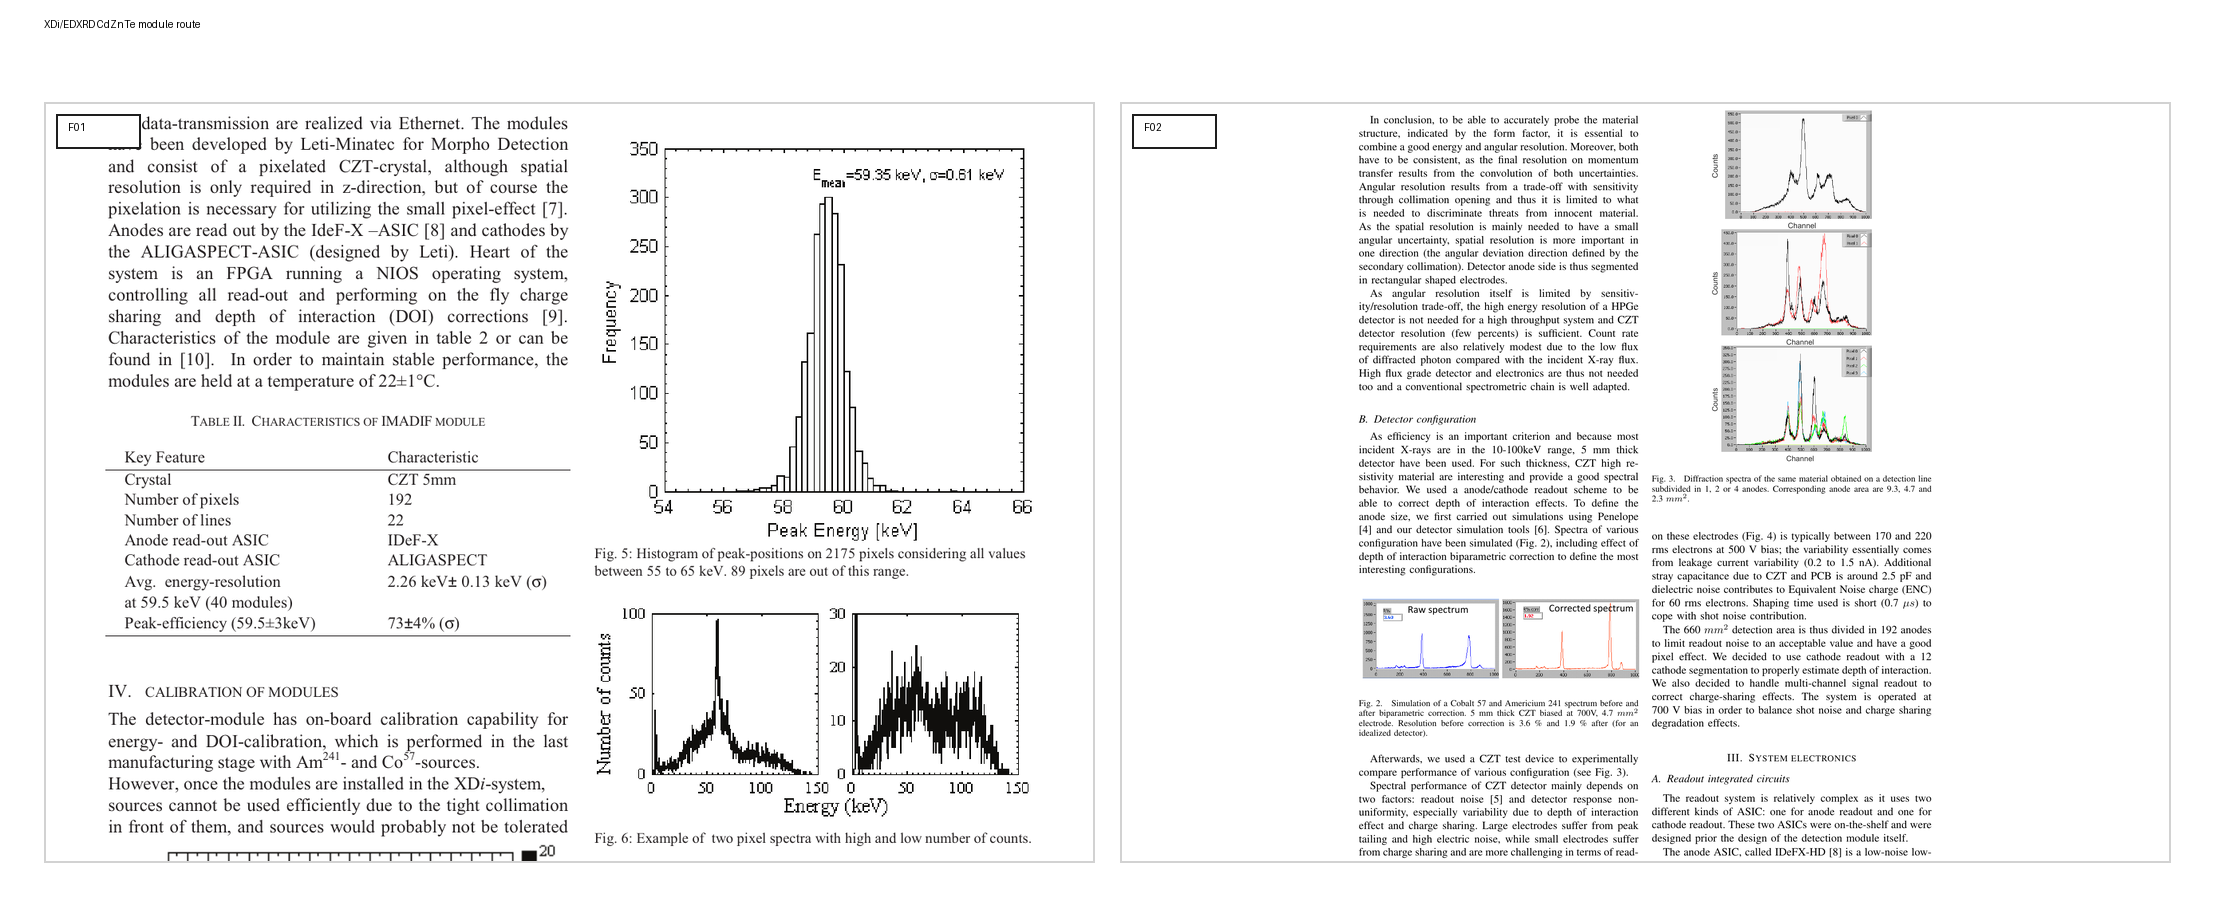
\includegraphics[width=\textwidth]{fig01_xdi_module.png}
  \caption{CEA-Leti/Morpho XDi/EDXRD 路线中的 CdZnTe 模块和系统温控证据。F01 中 $22\pm1\,\degc$ 是 XDi 模块内部温度，由模块内 dedicated sensor 读出；系统用长冷却板从下方控温，并通过约 $0.5\,\degc$ cooling-plate 步进验证峰位温漂。F02 中 $25\,\degc$ 是自主 CZT 模块调节温度，提取材料未给独立晶体温度传感位置。该路线的温控对象是模块/读出链，而非深冷晶体；目的在于保证多模块峰位、阈值和标定一致性\cite{kosciesza2013,montemont2013}。}
  \label{fig:xdi}
\end{figure*}

\section{温度影响探测器性能的主要通道}

\subsection{漏电流、噪声和前端余量}

温度升高通常增加体漏电、表面漏电和接触注入电流。漏电流通过 shot noise 增加等效噪声电荷，同时占用 ASIC 漏电补偿范围，并使低能阈值和基线校正更加困难。后文图~\ref{fig:cdtemech} 的 Principato 证据把这个量级具体化：在 Peltier thermal stage 控制的 CdTe 样品/探测器温度下，$-1000\,\mathrm{V}$ pixel current 从 $-25\,\degc$ 的约 $2\,\mathrm{pA}$ 上升到 $40\,\degc$ 的约 $3\,\mathrm{nA}$，差异接近三个数量级\cite{principato2012}。Thomas 等的 Redlen high-flux CdZnTe/PIXIE 测试也说明，ASIC 漏电补偿约 $250\,\mathrm{pA/pixel}$，漏电不是抽象材料参数，而会直接限制高增益模式和可用偏压\cite{thomas2017}。

对 XRD/EDXRD，漏电和噪声的重要性不只在 FWHM。峰位、谱尾和阈值漂移会改变散射谱的相对强度，进而影响物质分类。图~\ref{fig:coded} 中 Greenberg 等的 coded-aperture XRD 模型显示，探测器能量分辨率从 $7\,\mathrm{keV}$ 改善到 $2.5\,\mathrm{keV}$ 可显著降低重建误差；该图本身不是温控实验，但它说明任何由温度引起的能量分辨率和谱尾变化，都会进入最终重建质量\cite{greenberg2014}。

\subsection{峰位漂移、空间电荷和极化}

温度改变陷阱俘获/退俘获速率，进而改变空间电荷分布和内部电场。图~\ref{fig:cztpolar} 中 CdZnTe 高通量极化的典型图像来自 Bale 和 Szeles：慢速空穴被快速俘获，在入射侧累积正空间电荷，形成 electric-field pinch point；电子漂移时间变长、寿命降低并复合，谱峰向低能漂移，阈值以上计数先饱和后下降。其验证实验改变的是 temperature-stabilized detector arrays 的阵列温度而非明确晶体内点温度；模型预测临界通量近似随偏压平方增加，并通过深能级退俘获时间呈强温度依赖\cite{bale2008}。

CdTe Schottky 的极化机制则更像偏压后缓慢建立的耗尽层/空间电荷问题。图~\ref{fig:cdtemech} 将 Toyama 和 Principato 的证据放在一起：Toyama 的温度是恒温箱中的 CdTe 探测器样品温度，temperature controller 稳定度约 $\pm0.2\,\degc$；Principato 的温度是 Peltier thermal stage 上的 CdTe 样品/探测器温度，稳定度约 $\pm0.1\,\degc$ 并通氮气防凝露。Toyama 深受主模型给出 $E_T-E_V=0.69\,\mathrm{eV}$，退俘获时间从 $0\,\degc$ 的 $4695\,\mathrm{min}$ 降至 $30\,\degc$ 的 $351\,\mathrm{min}$；在 $20\,\degc$、$100\,\mathrm{V}$ 下，阴极侧电场约 $61\,\mathrm{min}$ 后达到零场，随后 depletion width 变窄并对应 $59.5\,\mathrm{keV}$ 光峰漂移\cite{toyama2006,principato2012}。

\begin{figure*}[t]
  \centering
  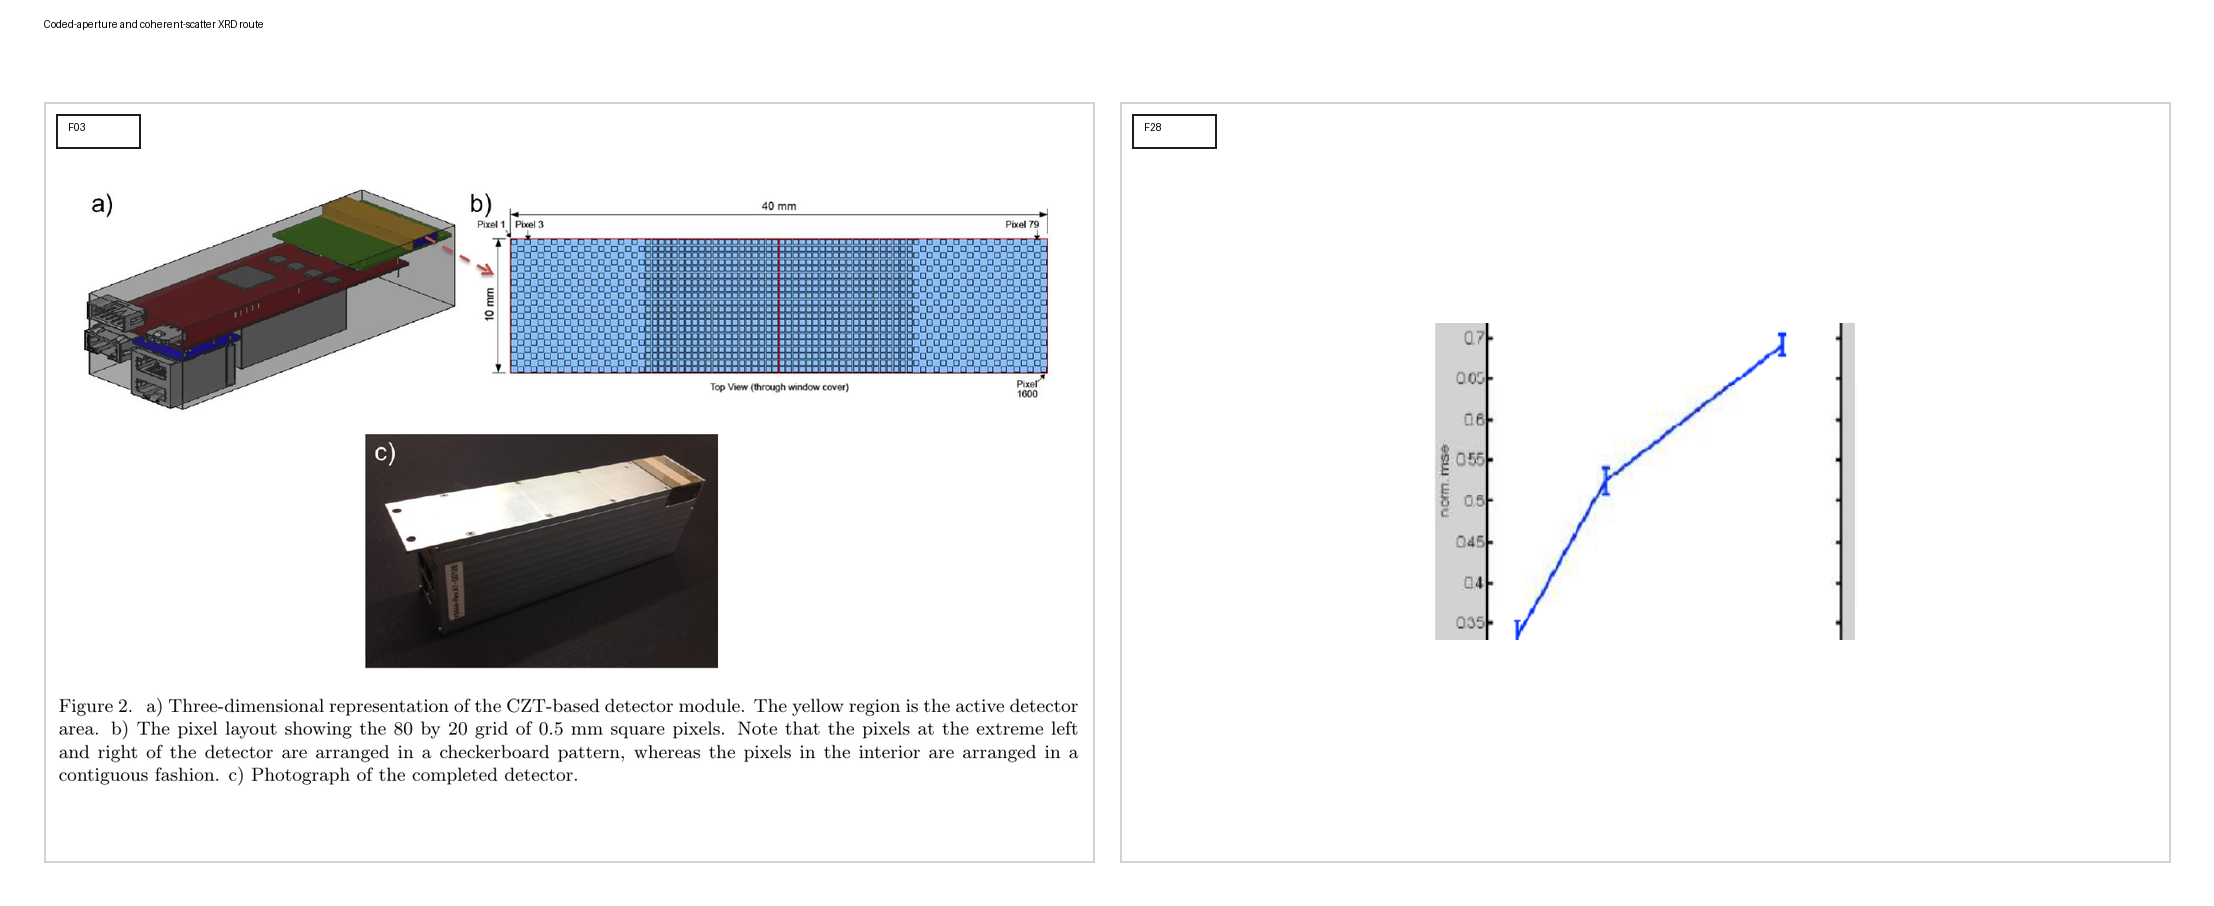
\includegraphics[width=\textwidth]{fig02_coded_aperture.png}
  \caption{Duke/Redlen coded-aperture 和 coherent-scatter XRD 路线。F03 显示中通量 CZT 光谱探测器需要把 ASIC 热源与 temperature-sensitive CZT 做结构/热隔离；该文只给室温/热隔离语境，未披露环境、板卡或晶体的具体温度测点。F28 是 coded-aperture XRD 模型图，不是温控实验；其证据意义是说明能量分辨率和谱尾会直接影响重建误差。Stryker 等后续 fan-beam 样机使用能量积分平板，本文只将其作为应用速度和几何路线参照，不作为 CdZnTe/CdTe 材料温度证据\cite{greenberg2014,greenberg2016,stryker2021}。}
  \label{fig:coded}
\end{figure*}

\subsection{长期稳定性和历史效应}

温控可以稳定当前工作点，却不能消除所有历史效应。图~\ref{fig:cdtestability} 中 CdTe 文献的 bias refresh、连续照射、前后响应图和漏电曲线都说明响应取决于此前偏压、剂量、空间照射分布和等待时间。Becker 等还显示，探测器/heat-sink 工作温度扫描中某些 delayed response 的衰减时间从 $+20\,\degc$ 的约 $90\,\mathrm{ms}$ 增加到 $-30\,\degc$ 的约 $150\,\mathrm{ms}$，说明降温虽然常降低漏电并延缓极化，但并非对所有时间响应指标单调有利\cite{becker2017}。

\section{CdZnTe：近室温稳定、高通量能力与接触工程}

CdZnTe 的系统优势首先体现在室温或轻度控温下的可用能谱稳定性。图~\ref{fig:xdi} 是系统级证据：CEA-Leti/Morpho 的自主 CZT XDi 模块以 room-temperature CZT 替代 cooled Ge，$5\,\mathrm{mm}$ 高阻 CdZnTe 与 IDeF-X/ALIGASPECT 读出组合在模块 $25\,\degc$ 调节条件下达到约 $3.8\%$ @ $60\,\mathrm{keV}$ 和 $2.4\%$ @ $122\,\mathrm{keV}$\cite{montemont2013}。后续 XDi 系统把 17 个模块置于长冷却板上，模块内 dedicated sensor 读出的温度控制在 $22\pm1\,\degc$，40 个模块平均达到 $2.26\pm0.13\,\mathrm{keV}$ @ $59.5\,\mathrm{keV}$，并给出约 $0.1\,\mathrm{keV}/\degc$ 的峰位温漂系数\cite{kosciesza2013}。这是一条产品化逻辑：温控不是为了追求深冷极限分辨率，而是为了让多模块峰位、阈值和标定在安检系统中保持一致。

图~\ref{fig:redlen} 和图~\ref{fig:hexitec} 把 Redlen HF-CdZnTe/HEXITEC 系列推向高通量问题。Veale 等在 $28\,\degc$ 和 $18\,\degc$ 对比条件下测试 Redlen HF-CdZnTe；这里温度更接近 ASIC/DAQ 控温点或探测器头/读出链设定，不是裸晶体直接测温。$28\,\degc$ 下 10 个器件平均约 $0.83\,\mathrm{keV}$ @ $59.54\,\mathrm{keV}$，且 9--12 小时内峰位、计数、charge sharing 和 FWHM 变化较小；$18\,\degc$ 下 FWHM 漂移更小，但这属于轻度降温而非深冷\cite{veale2020}。Cline 等在 HEXITEC MHz 中使用 $20\,\degc$ ASIC temperature、Peltier、湿控箱和外置除湿模块，证明 $>10^6\,\mathrm{ph\,s^{-1}\,mm^{-2}}$ 条件下仍可做能谱成像，同时发现局域 excess leakage-current 和基线偏移，提示高通量 CdZnTe 仍需要实时 offset correction 和湿温管理\cite{cline2024}。

\begin{figure*}[t]
  \centering
  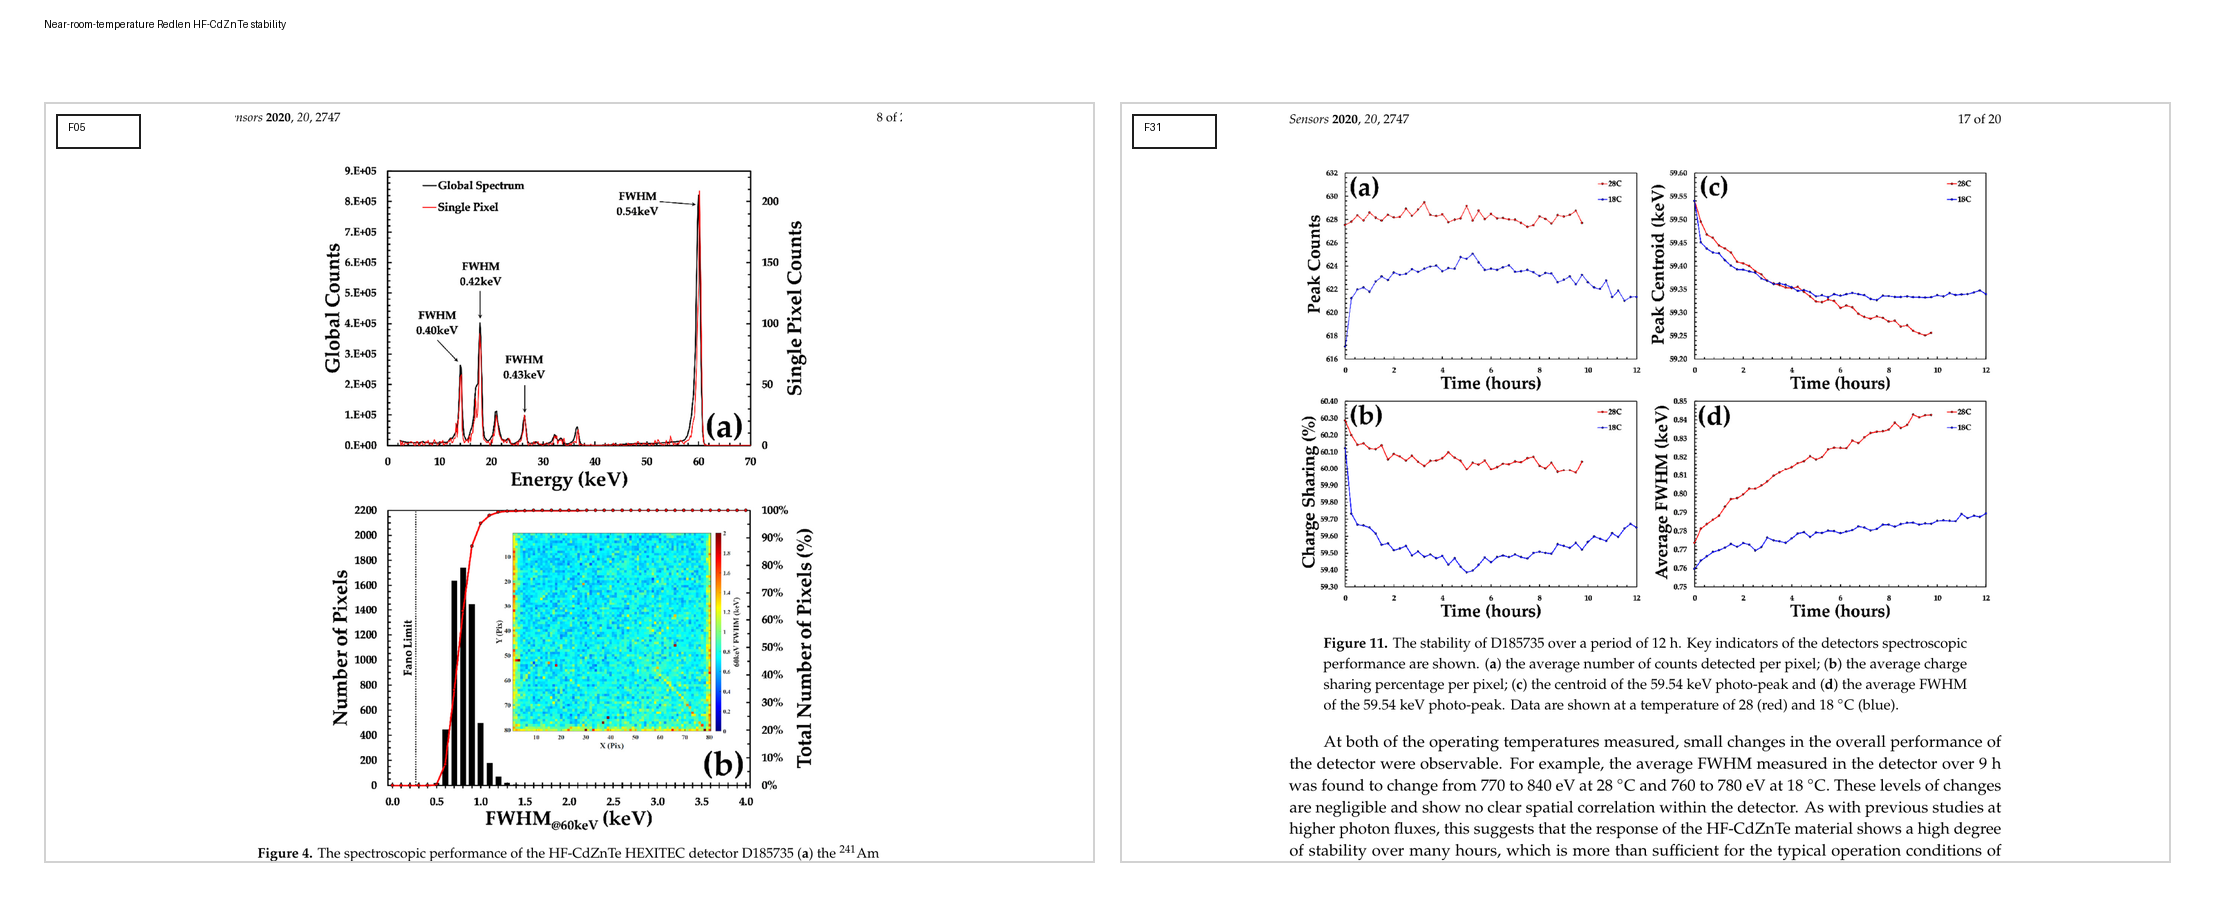
\includegraphics[width=\textwidth]{fig03_redlen_stability.png}
  \caption{Redlen HF-CdZnTe 的近室温谱学稳定性。F05 显示 HEXITEC/Redlen HF-CdZnTe 的 $^{241}$Am 能谱和 FWHM 均匀性；F31 显示 $28\,\degc$ 与 $18\,\degc$ 下 9--12 小时稳定性。这两个温度应按 HEXITEC GigE DAQ/ASIC 或探测器头设定温度理解，文献没有给出裸 CdZnTe 晶体内部温度传感位置。证据指向：轻度降温可减小 FWHM 漂移，但 $28\,\degc$ 系统设定下也已表现出可用长期稳定性\cite{veale2020}。}
  \label{fig:redlen}
\end{figure*}

高通量 CdZnTe 的材料级核心是空穴输运和接触工程，而不是单纯降温。Thomas 等在 $303\pm1\,\mathrm{K}$、RH $<10\%$ 条件下表征 Redlen high-flux CdZnTe，发现其电子 $\mu\tau$ 低于标准光谱级材料，但空穴 $\mu\tau$ 约 $2.9\times10^{-4}\,\mathrm{cm^2/V}$，较标准 Redlen 材料提高一个数量级以上\cite{thomas2017}。Prokesch 等的 eV Products THM CdZnTe 在 $23$--$28\,\degc$、$900\,\mathrm{V}$ 下承受最高约 $10^8\,\mathrm{photons\,mm^{-2}\,s^{-1}}$ 入射通量而无电场极化；对照低通量光谱级 CZT 虽有更好电子 $\mu\tau$，却因空穴 $\mu\tau$ 低而在 $<1\,\mathrm{Mcps/mm^2}$ 即极化\cite{prokesch2016}。

图~\ref{fig:cztpolar} 的第三个证据来自 Baussens 等：Redlen HF-CZT 使用优化 Au/Pt 和 Pt/Pt 接触，$20\,\degc$ 是 Julabo FL300 循环冷却器和 Pt100 读出的样品/平台温度，并用氮气流防凝露；该条件下暗电流密度约 $90$ 和 $60\,\mathrm{pA/mm^2}$，并在 $20\,\mathrm{keV}$、$3\times10^7$--$8\times10^9\,\mathrm{photons\,mm^{-2}\,s^{-1}}$ 范围内保持 $R^2>0.999$ 的光电流线性；Pt/Pt 样品可测试到 $10^{12}\,\mathrm{photons\,mm^{-2}\,s^{-1}}$，但 $>10^{11}\,\mathrm{photons\,mm^{-2}\,s^{-1}}$ 出现 hysteresis\cite{baussens2022}。Bettelli 等进一步证明 Pt/CdTeO$_3$/CZT 界面可以阻挡空穴注入并利于抽取，使 Pt 阳极样品在约 $500\,\mathrm{V/mm}$ 下维持约 $40\,\mathrm{pA/mm^2}$ 漏电密度，在 $1200\,\mathrm{V/mm}$ 下仍可控制在约 $300\,\mathrm{pA/mm^2}$\cite{bettelli2023}。因此，对 CdZnTe 而言，最佳工程路线通常是中等温控、低漏电接触、高偏压和高空穴输运协同。

\begin{figure*}[t]
  \centering
  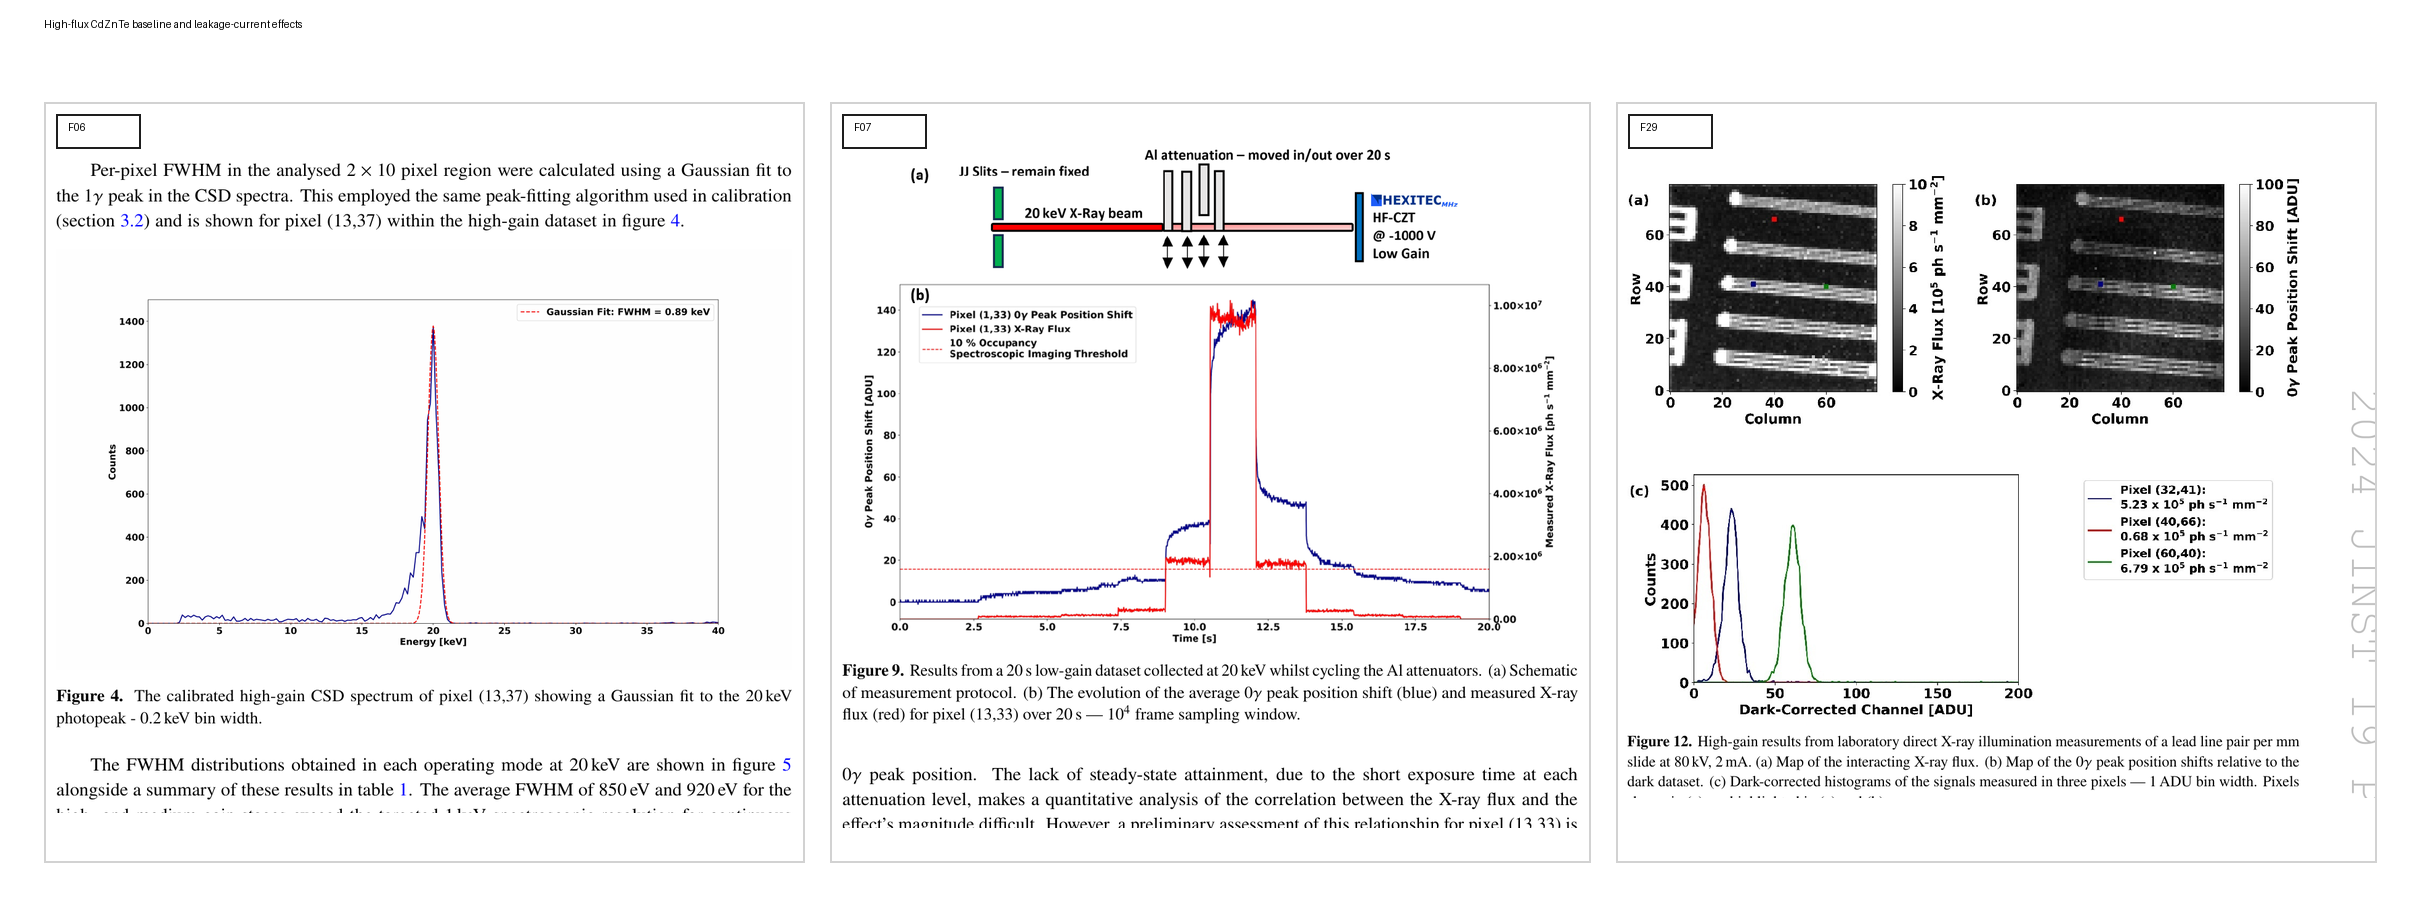
\includegraphics[width=\textwidth]{fig04_hexitec_mhz.png}
  \caption{HEXITEC MHz 高通量 CdZnTe 中的基线和漏电流效应。F06 显示 $20\,\mathrm{keV}$ 高增益谱峰仍可得到约 $850\,\mathrm{eV}$ FWHM；F07 和 F29 显示高通量照射下的 0-gamma peak shift、空间局域基线偏移和 excess leakage-current。文中温度写作 ASIC temperature $20\,\degc$：探测器安装在 Peltier 上，LOKI/PCB 传感器监测温湿度，电源反馈维持稳定，低于环境时用 solid-state dehumidifiers 防凝露；因此该温度口径主要是 ASIC/板卡温度，不是裸晶体直接读数。该效应不是传统 bulk polarization，但会进入峰位和阈值稳定性预算\cite{cline2024}。}
  \label{fig:hexitec}
\end{figure*}

\begin{figure*}[t]
  \centering
  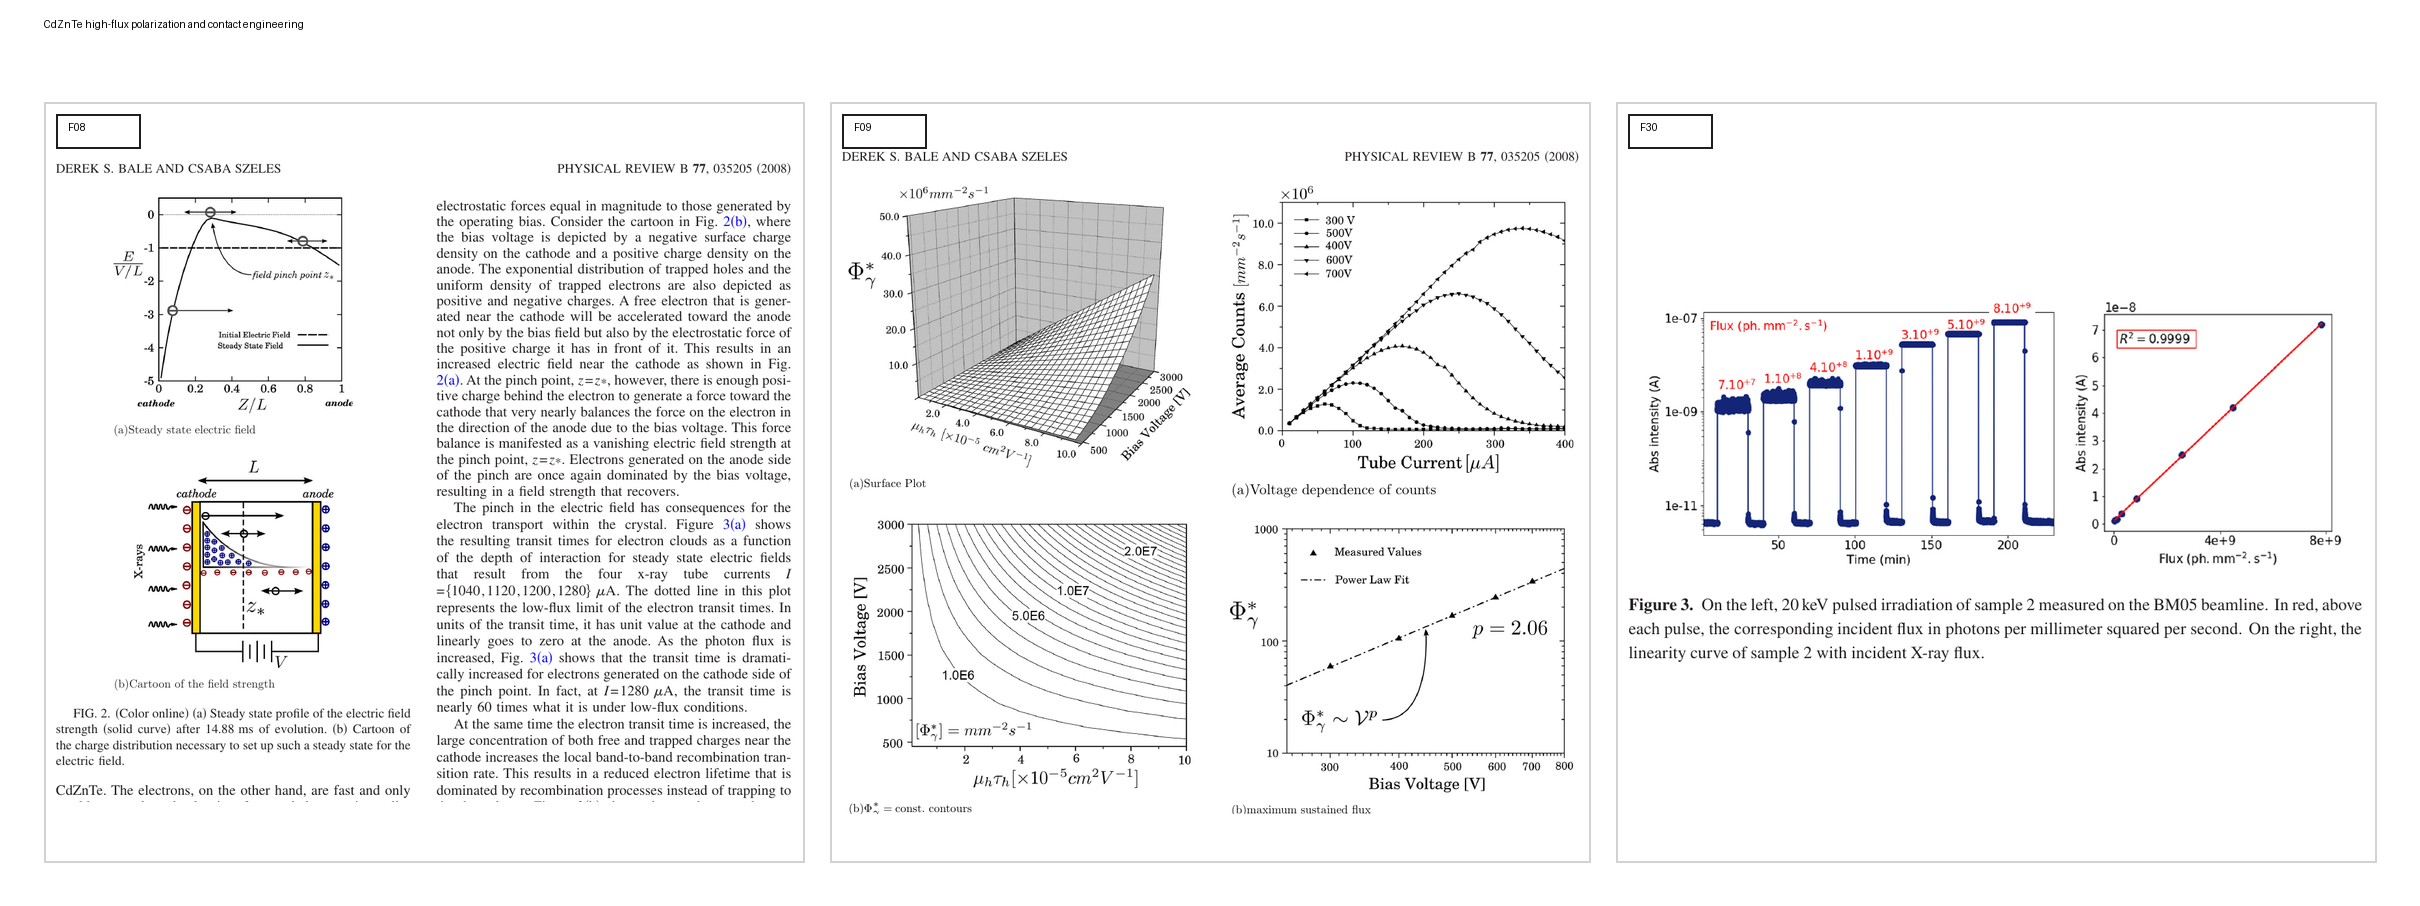
\includegraphics[width=\textwidth]{fig05_czt_polarization_contacts.png}
  \caption{CdZnTe 高通量极化和接触工程。F08/F09 给出 Bale--Szeles 模型和临界通量的偏压/温度依赖；其实验温度是 temperature-stabilized CdZnTe detector arrays 的阵列温度，验证实验固定 $900\,\mathrm{V}$ 并改变 $15$--$45\,\degc$，但提取材料未给出晶体内部传感位置。F30 显示优化电极 Redlen HF-CdZnTe 在 $20\,\degc$ 同步辐射高通量照射下的线性和稳定性；该温度由 Julabo 冷却器和 Pt100 作为样品/平台温度读出，并有氮气防凝露。图组强调：温度、偏压、空穴输运和接触注入必须一起设计\cite{bale2008,baussens2022}。}
  \label{fig:cztpolar}
\end{figure*}

\section{CdTe：低温、偏压刷新与极化历史}

CdTe 的高 $Z$ 和成熟晶体工艺使其成为 CdZnTe 的重要对照，但 Schottky CdTe 的温度敏感性更强。图~\ref{fig:cdtemech} 是机理证据：Toyama 和 Principato 的结果共同说明，CdTe Schottky 的极化并非单纯电子噪声问题，而是深受主退俘获、空间电荷、电场重构和偏压后等待时间共同作用的结果\cite{toyama2006,principato2012}。Principato 等特别指出，Al/p-CdTe/Pt 的 I-V 曲线在 $1\,\mathrm{ms}$--$1000\,\mathrm{s}$ 时间尺度内都有时间依赖，即使 $<1\,\mathrm{s}$ 的测量延迟也会改变测得电流；因此，如果不说明偏压后等待时间和温度测点，CdTe 漏电数据很难横向比较\cite{principato2012}。

图~\ref{fig:cdtestability} 是 CdTe 稳定性证据，说明低温 CdTe 可以获得稳定能谱，但工程代价明显更高。Minami 等的 $2\,\mathrm{mm}$ 厚 CdTe DSD 在 $-20\,\degc$、$500\,\mathrm{V}$ 下实现 $2.6\,\mathrm{keV}$ @ $122\,\mathrm{keV}$ 和 $4.3\,\mathrm{keV}$ @ $356\,\mathrm{keV}$，并在约 20 小时内能量分辨率变化 $<1\%$；该 $-20\,\degc$ 是探测器低温工作点，提取材料未详述测温位置\cite{minami2023}。Franklin 等的 electron-collecting Acrorad CdTe 使用真空封装、透明窗口和 TEC $\pm0.1\,\degc$，其 $0/20\,\degc$ 是 sensor temperature，较接近探测器/晶体温度口径；更高温度和更低偏压会加快极化\cite{franklin2024}。Becker 等选择 $0\,\degc$ 作为主要工作点，说明低温和高电压可缩短偏压建立后的稳定时间，但 persistence 释放时间在低温下变长\cite{becker2017}。

\begin{figure*}[t]
  \centering
  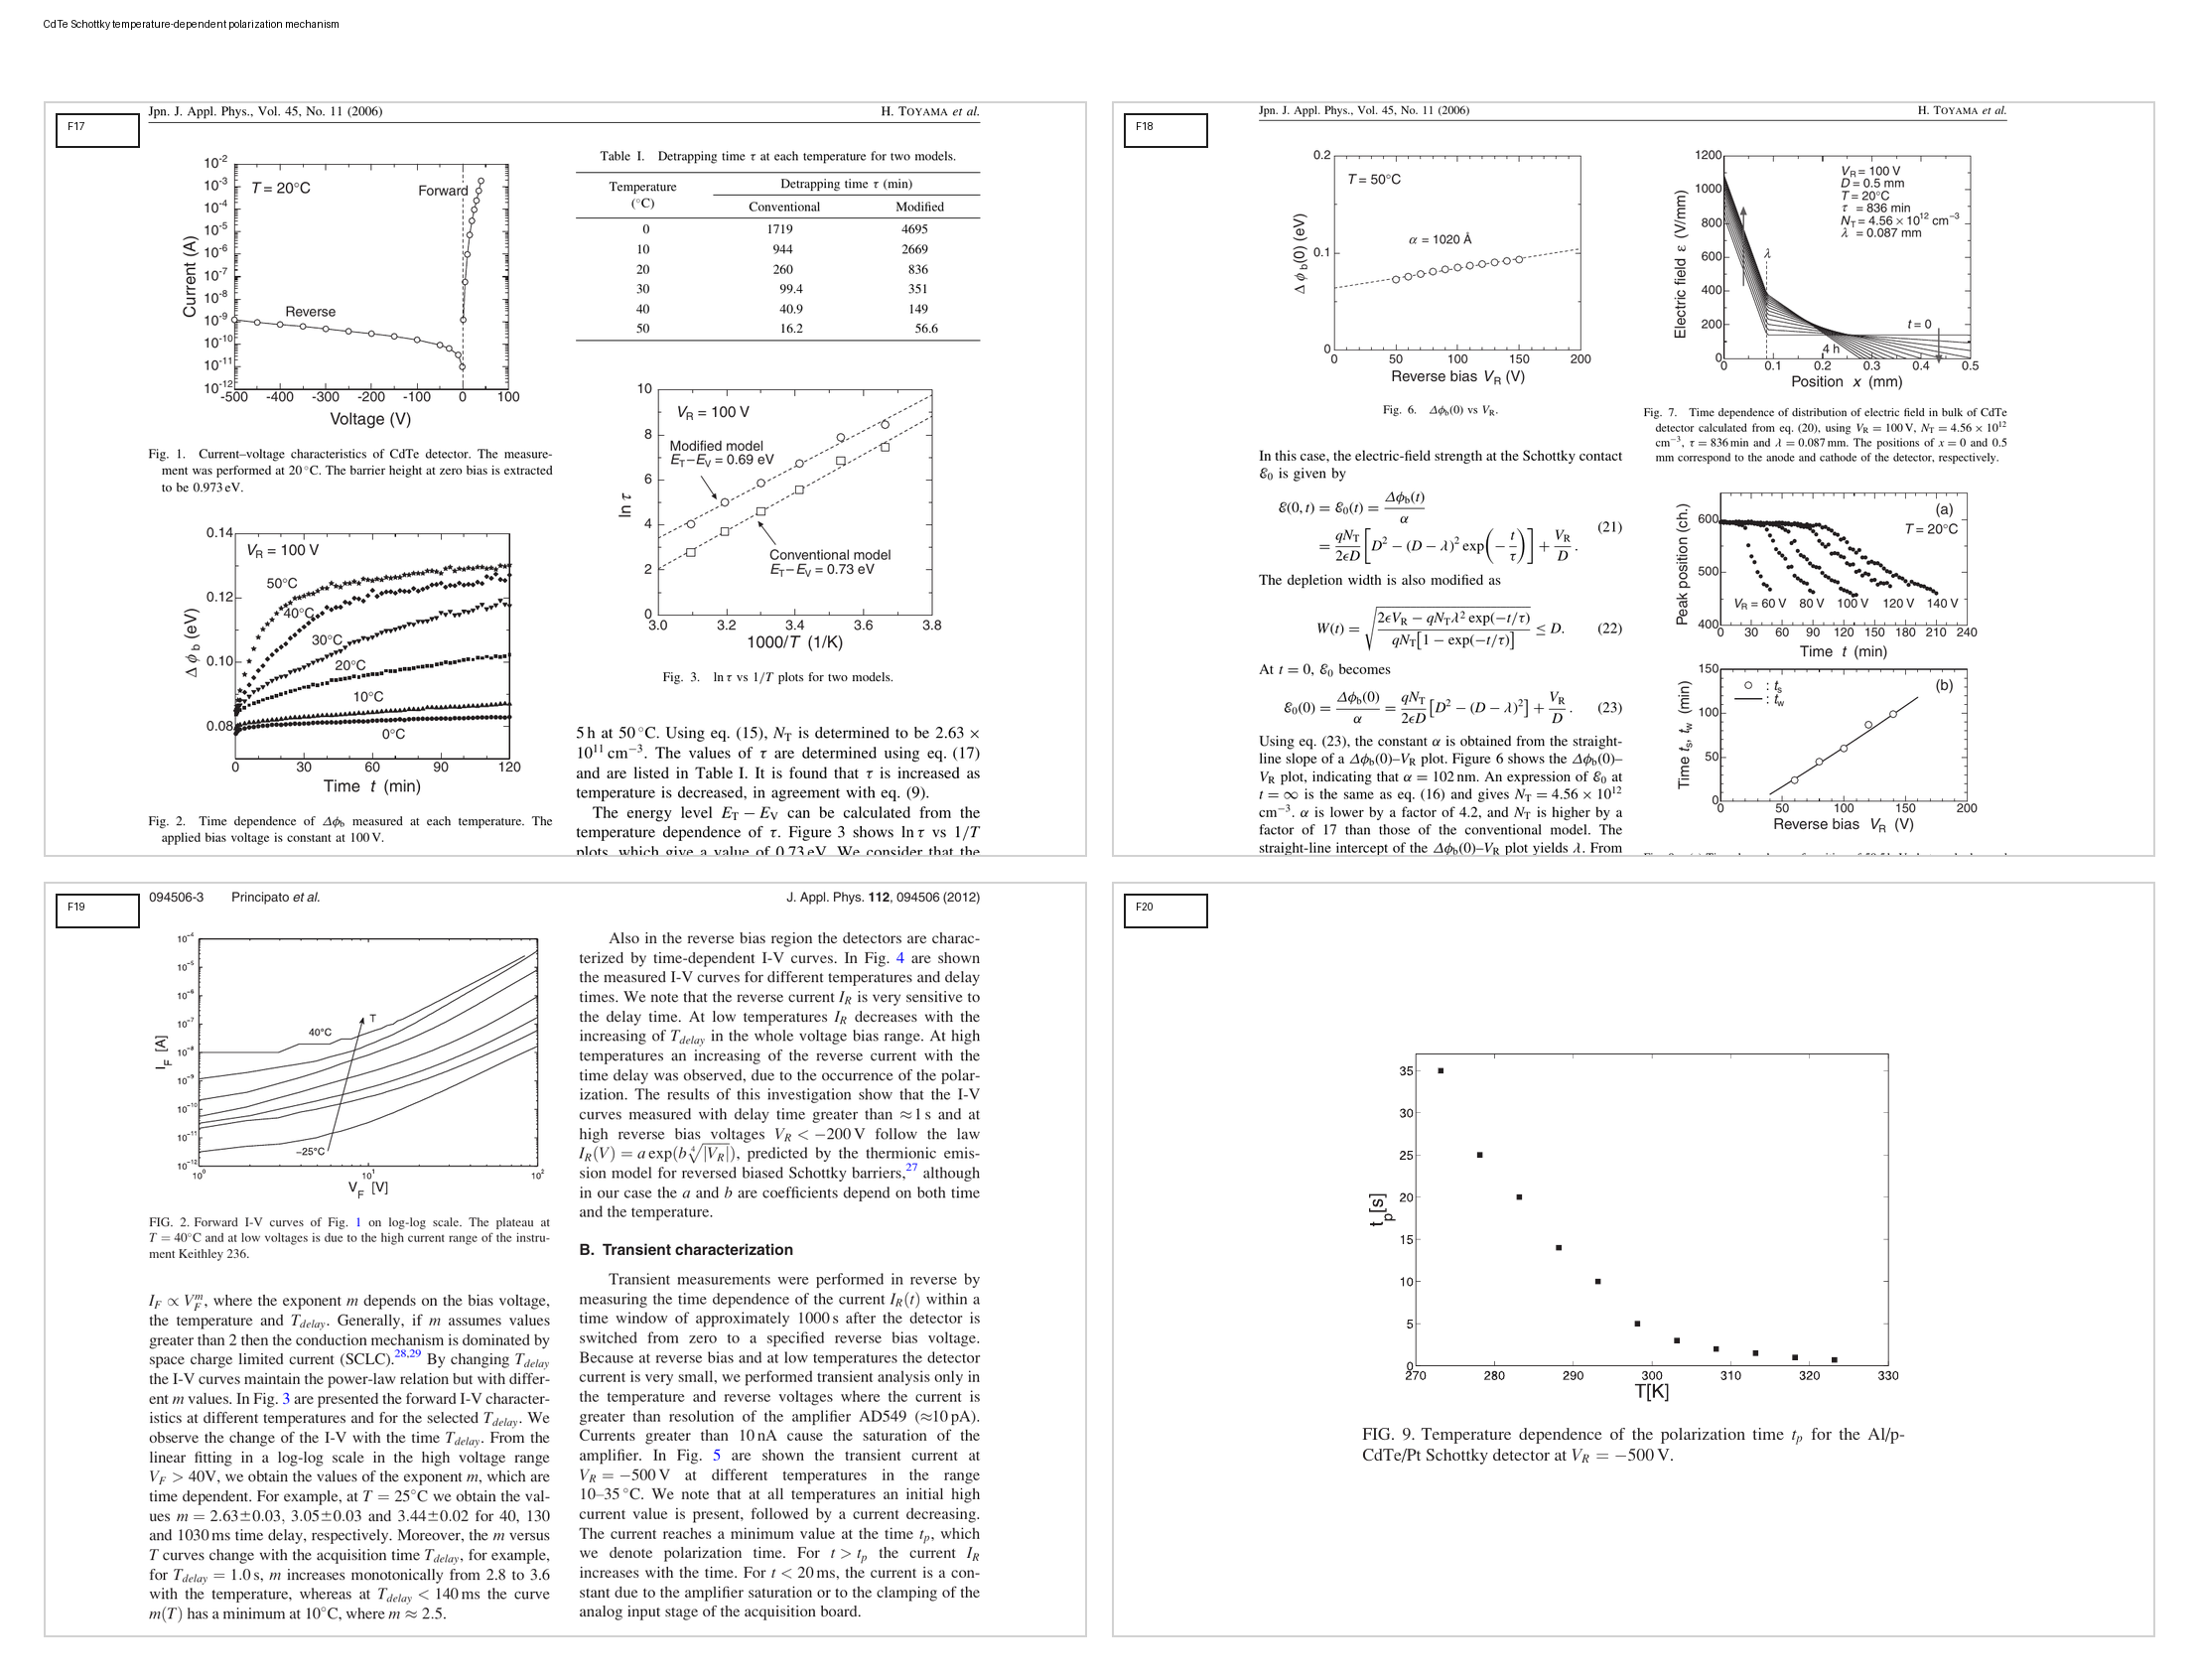
\includegraphics[width=\textwidth]{fig06_cdte_mechanism.png}
  \caption{CdTe Schottky 的温度依赖极化机制。F17/F18 来自 Toyama：温度是恒温箱中的 CdTe 探测器样品温度，temperature controller 稳定度约 $\pm0.2\,\degc$，I-V 扫描 $0$--$50\,\degc$、谱测试 $20\,\degc$，图中连接深受主退俘获、电场分布和 $59.5\,\mathrm{keV}$ 峰位漂移。F19/F20 来自 Principato：温度是 Peltier thermal stage 上的 Al/p-CdTe/Pt 样品/探测器温度，稳定度约 $\pm0.1\,\degc$，并通氮气防凝露；I-V 温度为 $-25$--$40\,\degc$，极化时间 $t_p$ 随温度降低而增加。该证据链解释了为什么 CdTe 文献常采用 Peltier、水冷、氮气或真空环境\cite{toyama2006,principato2012}。}
  \label{fig:cdtemech}
\end{figure*}

CdTe 的高通量和连续照射稳定性尤其需要谨慎。图~\ref{fig:cdtestability} 同时放入 Meyer、Franklin 和 Astromskas 的证据，是因为三者分别对应水冷模块、真空 TEC sensor temperature 和 MERLIN/冷板模块温度。Astromskas 等在 Acrorad Schottky CdTe/Medipix3RX 中发现，温度、通量和曝光时间共同控制极化速度；其温度应按 water chiller+copper plate 附近的探测器模块/冷板温度理解，并由 MERLIN 系统监测而非明确晶体内部读数。高通量下出现 tri-phase pixel 行为，bias reset 可以恢复初始响应，但 $300\,\mathrm{kcps/pixel}$ 条件下需要约 $15$--$20\,\mathrm{s}$ off-time 才足以稳定\cite{astromskas2016}。Meyer 等用 JUNGFRAU 读出比较 Acrorad Schottky 与 ohmic CdTe：$0\,\degc$、$-500\,\mathrm{V}$、低通量下 5 小时几乎无极化，$+15\,\degc$ 约 $200\,\mathrm{min}$ 出现极化，$+30\,\degc$ 约 $35\,\mathrm{min}$ 开始极化，约 $70\,\mathrm{min}$ 后 $99\%$ pixels 低于初始平均计数的 $50\%$\cite{meyer2022}。预辐照区域更抗极化，但代价是漏电升高；热退火也会改变后续极化过程。这些结果显示，CdTe 系统必须把温度、偏压刷新、剂量历史和接触结构作为一个整体设计。

\begin{figure*}[t]
  \centering
  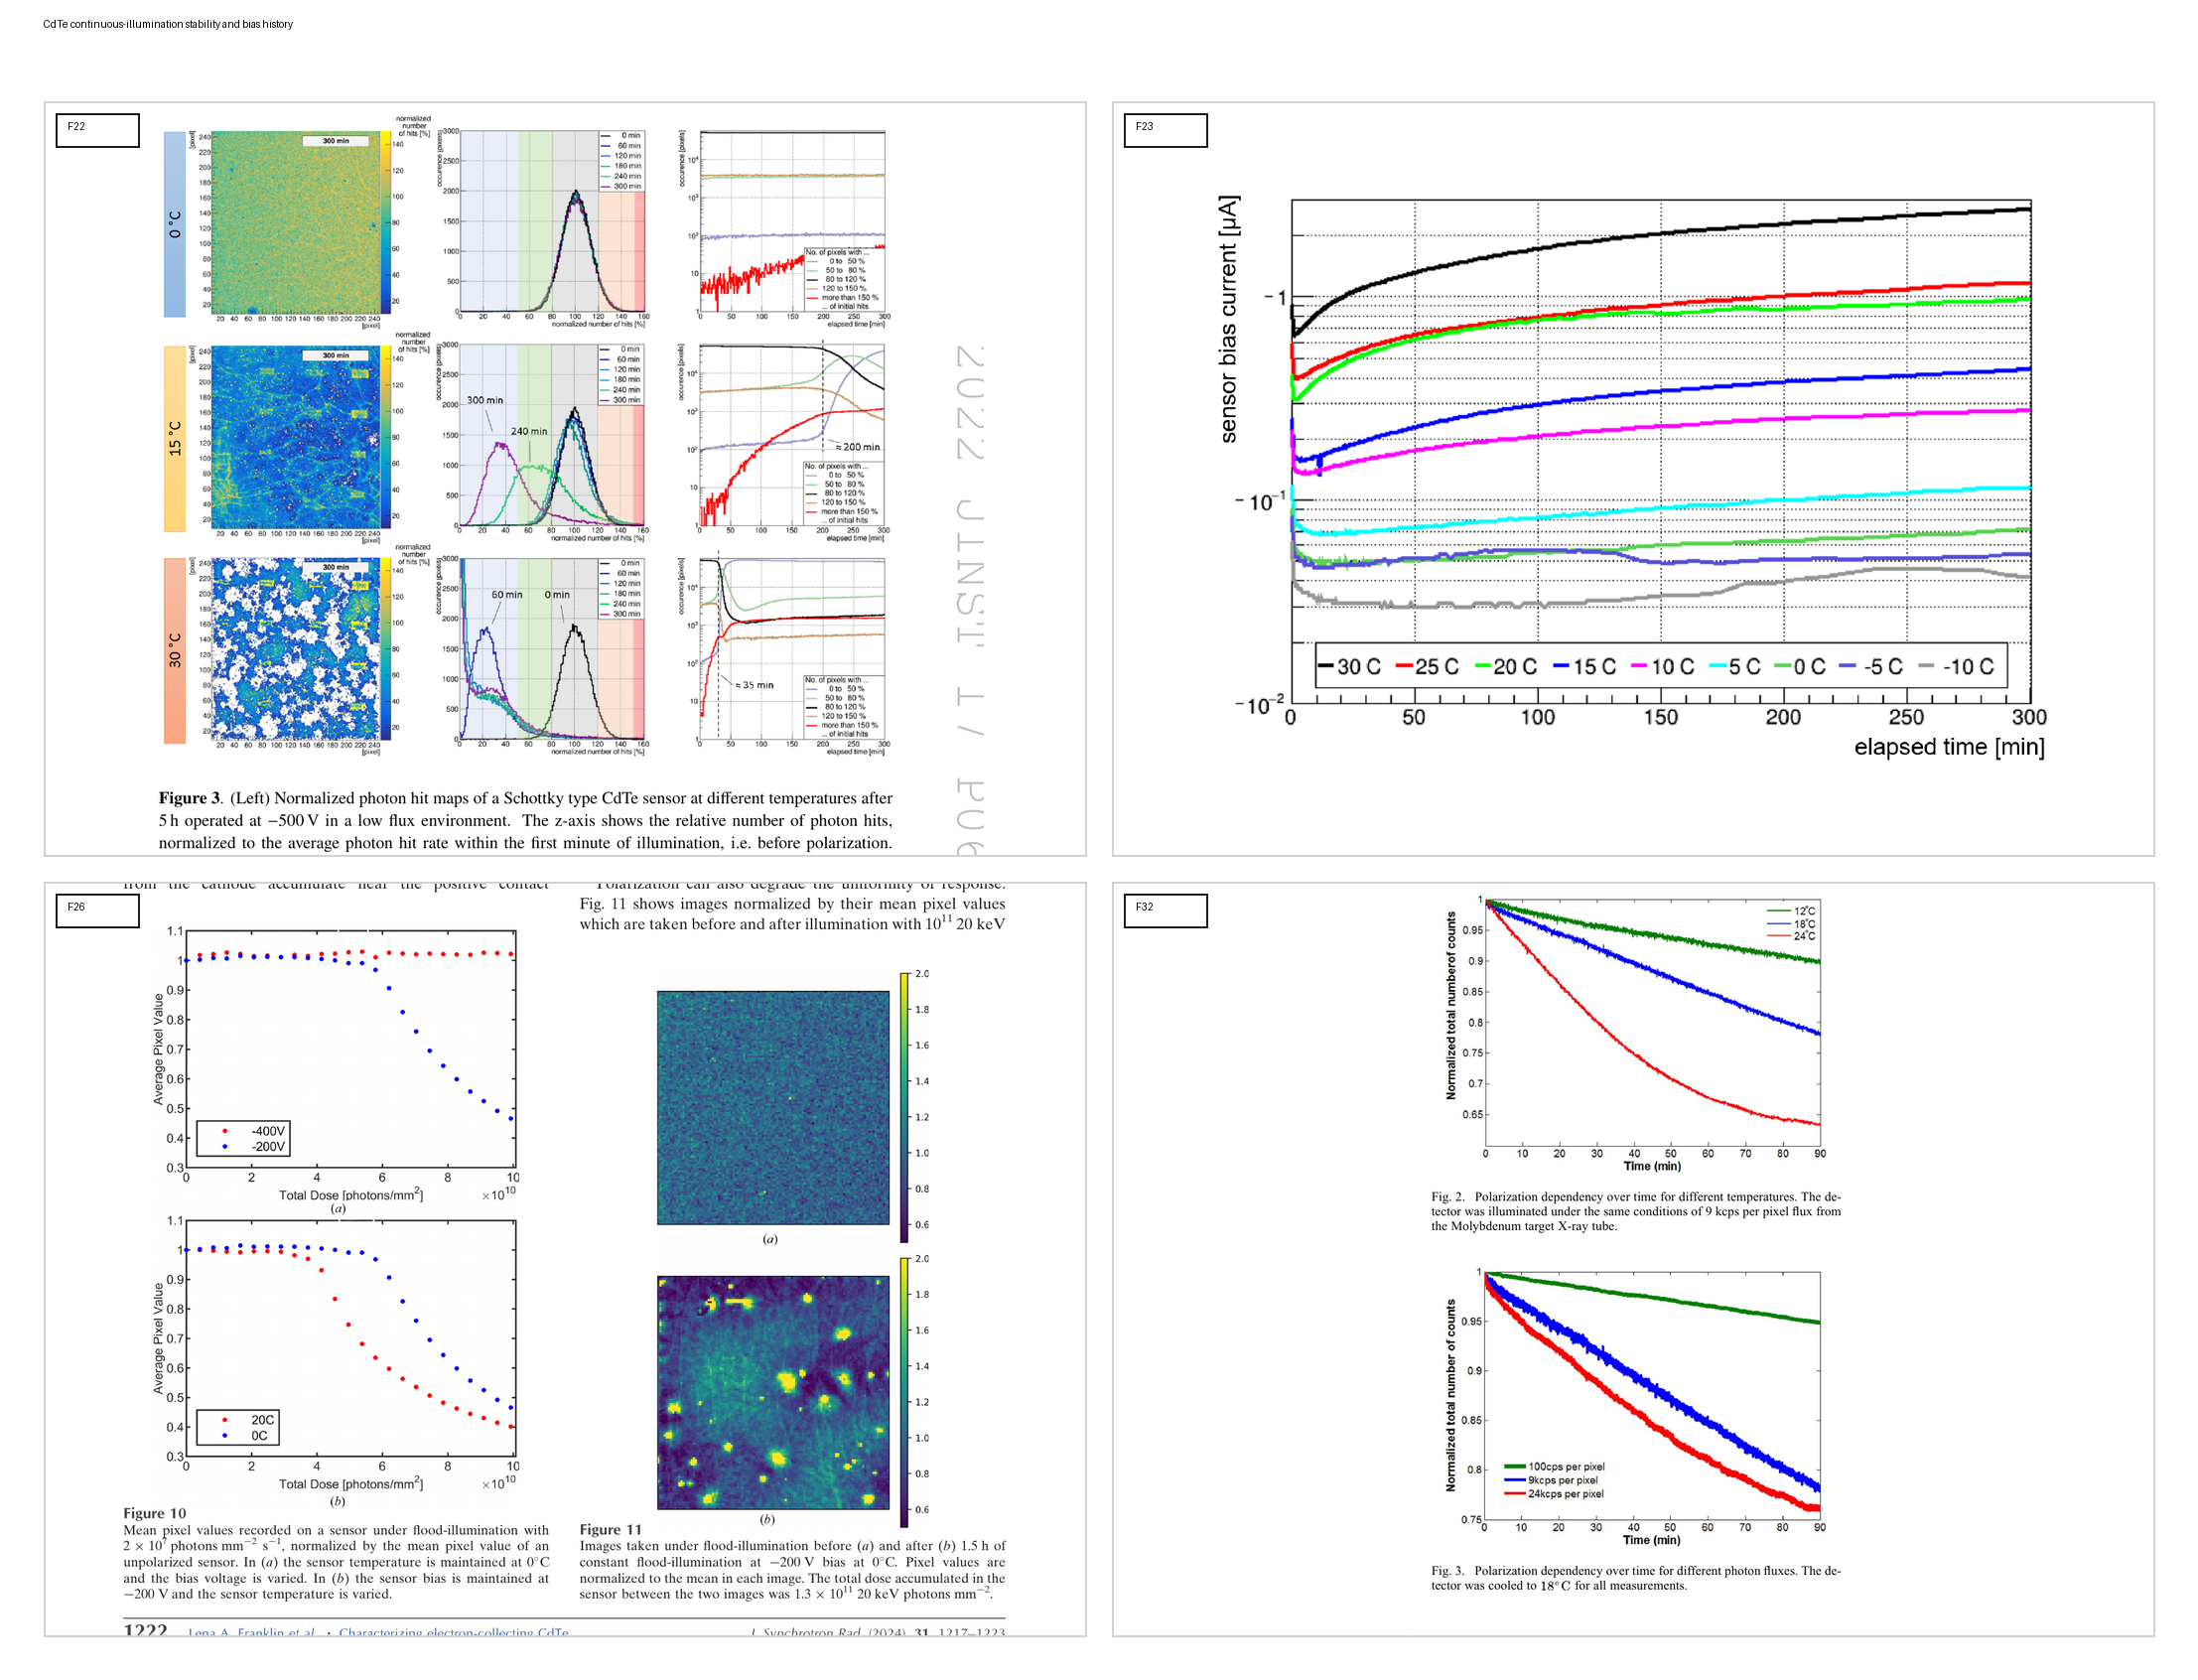
\includegraphics[width=\textwidth]{fig07_cdte_stability.png}
  \caption{CdTe 连续照射稳定性和偏压历史。F22/F23 显示 Meyer 的 Acrorad Schottky CdTe 在 $0/15/30\,\degc$ 下连续照射后的计数图和漏电演化；该温度是水冷系统控制的探测器/前端模块设定温度，稳定度约 $\pm0.1\,\mathrm{K}$，并用氮气流防凝露。F26 显示 Franklin 的 electron-collecting CdTe 中低温和高偏压延缓极化；其 $0/20\,\degc$ 是 evacuated housing 内 TEC 控制的 sensor temperature，稳定度约 $\pm0.1\,\degc$。F32 显示 Astromskas 的 Medipix3RX Schottky CdTe 极化随温度和通量加速；其 $12/18/24\,\degc$ 应按 water chiller+copper plate/MERLIN 监测的探测器模块或冷板附近温度理解，而不是晶体内部点温。该图组支持 CdTe 更依赖低温、封装和刷新策略的判断\cite{meyer2022,franklin2024,astromskas2016}。}
  \label{fig:cdtestability}
\end{figure*}

\section{温控工程方案与公司路线}

表~\ref{tab:temperature} 汇总了本文关心的三类温控逻辑。第一类是 CdZnTe 安检/EDXRD 模块的室温恒温，例如 XDi 的 $22\pm1\,\degc$ 或模块级 $25\,\degc$。收益是峰位漂移可控、多模块可标定、无需 Ge 深冷真空系统；代价是冷却板、温度传感器、系统标定和低于环境运行时的凝露管理\cite{kosciesza2013,montemont2013}。第二类是 high-flux CdZnTe 的 $18$--$30\,\degc$ 轻度控温，常见 Peltier、recirculating chiller、Pt100、湿度控制、氮气或除湿模块。收益是稳定 ASIC、漏电、偏压和基线，同时允许高场工作；代价是功耗、体积、温度梯度和机械封装复杂度\cite{cline2024,baussens2022,bettelli2023}。第三类是 CdTe Schottky 的低温/TEC/水冷路线，收益是降低漏电并延缓极化，代价是凝露、真空/氮气、防冷凝窗口、bias refresh 死时间和维护复杂度\cite{minami2023,franklin2024,meyer2022,principato2012}。

\begin{table*}[t]
\caption{CdZnTe/CdTe 温度响应和温控工程路线对比。}
\label{tab:temperature}
\centering
\small
\renewcommand{\arraystretch}{1.18}
\begin{tabular}{@{}lllll@{}}
\toprule
\tcell[0.15\textwidth]{路线} & \tcell[0.14\textwidth]{典型温度} & \tcell[0.20\textwidth]{主要收益} & \tcell[0.22\textwidth]{主要代价} & \tcell[0.18\textwidth]{代表文献} \\
\midrule
\tcell[0.15\textwidth]{CdZnTe XDi/EDXRD} & \tcell[0.14\textwidth]{$22\pm1\,\degc$ 或 $25\,\degc$} & \tcell[0.20\textwidth]{峰位一致、多模块标定、替代 Ge 深冷} & \tcell[0.22\textwidth]{冷却板、传感器、凝露和系统标定} & \tcell[0.18\textwidth]{CEA-Leti\\Morpho\\Smiths\cite{kosciesza2013,montemont2013}} \\
\tcell[0.15\textwidth]{Redlen/eV high-flux CdZnTe} & \tcell[0.14\textwidth]{$18$--$30\,\degc$，常见 $20\,\degc$} & \tcell[0.20\textwidth]{高偏压低漏电、ASIC/基线稳定、高通量抗极化} & \tcell[0.22\textwidth]{Peltier/chiller/氮气/除湿、体积功耗增加} & \tcell[0.18\textwidth]{Redlen/Canon, eV/Kromek, ESRF/IMEM-CNR\cite{veale2020,cline2024,prokesch2016,baussens2022,bettelli2023}} \\
\tcell[0.15\textwidth]{Acrorad CdTe Schottky} & \tcell[0.14\textwidth]{$-20$--$0\,\degc$ 常见，也常测试 $0/15/30\,\degc$} & \tcell[0.20\textwidth]{降低漏电、延缓极化、允许较高偏压} & \tcell[0.22\textwidth]{TEC/水冷、真空或氮气、防凝露、bias reset 死时间} & \tcell[0.18\textwidth]{Acrorad CdTe\\JUNGFRAU\\Medipix\\DSD\cite{astromskas2016,becker2017,meyer2022,minami2023,franklin2024}} \\
\bottomrule
\end{tabular}
\end{table*}

CEA-Leti/Morpho/Smiths Detection 的 XDi 路线代表产品化 EDXRD 安检系统。该路线选择像素化 CdZnTe 模块、室温/轻度恒温、可替换模块和系统级标定。$22\pm1\,\degc$、$0.1\,\mathrm{keV}/\degc$ 和 $2.26\,\mathrm{keV}$ @ $59.5\,\mathrm{keV}$ 等指标说明，温控在这里是谱峰一致性和长期可维护性的工具，而不是把探测器推向极限能量分辨率\cite{kosciesza2013,montemont2013}。

Duke/Redlen coded-aperture/coherent scatter 路线代表算法和几何编码驱动的 XRD 系统。Greenberg 2016 的 Redlen CZT 探测器在中通量 coherent scatter 中直接面对 ASIC 发热、CZT 温度敏感性和热/结构隔离问题\cite{greenberg2016}。Stryker 2021 的 fan-beam 样机使用能量积分平板，不应被误写为 CdZnTe/CdTe 样机；它的价值在于说明系统速度、SNR 和 $q$ 分辨率是最终约束，若未来换成 CdZnTe/CdTe 能谱探测器，温控会直接进入速度和谱准确性的权衡\cite{stryker2021}。

Redlen/Canon 与 eV Products/Kromek 线索共同说明 CdZnTe 的商业化高通量路线。前者在 HEXITEC、同步辐射和 high-flux 材料均匀性中体现为 Redlen HF-CZT；后者在 Prokesch 和 Bale/Szeles 中体现为 THM CdZnTe 和高通量极化模型\cite{veale2020,thomas2017,prokesch2016,bale2008}。Acrorad 则是 CdTe 对照文献的主要材料来源，其优势是成熟 CdTe Schottky/ohmic 器件和高效率，弱点是低温、偏压刷新和极化历史管理更重\cite{astromskas2016,meyer2022,franklin2024}。ESRF/IMEM-CNR/Bettelli/Baussens 线索显示，接触工程正在把 high-flux CdZnTe 推向同步辐射/FEL 的极高通量直接探测\cite{baussens2022,bettelli2023,greiffenberg2025}。

\begin{table*}[t]
\caption{面向 XRD/EDXRD 和能谱成像的代表性系统路线。}
\label{tab:routes}
\centering
\small
\renewcommand{\arraystretch}{1.18}
\begin{tabular}{@{}lllll@{}}
\toprule
\tcell[0.16\textwidth]{机构/公司路线} & \tcell[0.11\textwidth]{材料} & \tcell[0.17\textwidth]{应用} & \tcell[0.24\textwidth]{温控/性能线索} & \tcell[0.21\textwidth]{综述中的作用} \\
\midrule
\tcell[0.16\textwidth]{CEA-Leti\\Morpho\\Smiths XDi} & \tcell[0.11\textwidth]{CdZnTe} & \tcell[0.17\textwidth]{EDXRD 安检} & \tcell[0.24\textwidth]{$22\pm1\,\degc$；$0.1\,\mathrm{keV}/\degc$；$2.26\,\mathrm{keV}$ @ $59.5\,\mathrm{keV}$} & \tcell[0.21\textwidth]{说明产品化系统为什么选择室温恒温 CdZnTe} \\
\tcell[0.16\textwidth]{Duke\\Redlen\\Quadridox} & \tcell[0.11\textwidth]{CdZnTe 或能量积分平板参照} & \tcell[0.17\textwidth]{coded-aperture/coherent scatter XRD} & \tcell[0.24\textwidth]{中通量 CZT 需热隔离；fan-beam 样机说明速度/SNR 约束} & \tcell[0.21\textwidth]{连接探测器温控与 XRD 重建质量} \\
\tcell[0.16\textwidth]{Redlen/Canon, eV/Kromek} & \tcell[0.11\textwidth]{CdZnTe} & \tcell[0.17\textwidth]{high-flux photon counting / synchrotron imaging} & \tcell[0.24\textwidth]{$18$--$30\,\degc$；高空穴输运；高偏压；接触工程} & \tcell[0.21\textwidth]{说明 CdZnTe 高通量路线不是单靠降温} \\
\tcell[0.16\textwidth]{Acrorad} & \tcell[0.11\textwidth]{CdTe} & \tcell[0.17\textwidth]{Medipix\\JUNGFRAU\\PAD\\DSD} & \tcell[0.24\textwidth]{$-20$--$0\,\degc$；TEC/水冷/真空/氮气；bias refresh} & \tcell[0.21\textwidth]{作为 CdTe 对照，突出低温和历史效应} \\
\bottomrule
\end{tabular}
\end{table*}

\section{综合判断}

第一，CdZnTe 更适合室温或轻度控温稳定工作，尤其当材料为空穴输运优化的 high-flux CdZnTe 且接触工程足够好时。温控的主要目标是稳定 ASIC、漏电、基线、峰位和多模块标定；在高通量极限下，温度仍通过空穴退俘获和空间电荷影响 critical flux，但单纯降温不能替代材料和接触工程\cite{bale2008,prokesch2016,veale2020,cline2024,greiffenberg2025}。

第二，CdTe 尤其 Schottky CdTe 更依赖低温、TEC/水冷、氮气或真空、防凝露和 bias refresh。温度对 CdTe 的影响不仅是漏电和噪声，还直接改变深受主退俘获、空间电荷建立、depletion width、峰位漂移和像素均匀性。$0\,\degc$ 与 $30\,\degc$ 的差异可以表现为数小时稳定与几十分钟极化的差异\cite{toyama2006,principato2012,astromskas2016,meyer2022}。

第三，降温不等于性能单调提升。对 CdTe，降温通常降低漏电并延缓极化，但可能延长 persistence 或增加偏压刷新、封装和防凝露成本；对 CdZnTe，高通量稳定性常由空穴 $\mu\tau$、偏压、厚度、接触注入、阈值和 ASIC 校正共同决定。最优温度应定义为工程最优区间：在可接受的功耗、体积、凝露风险和维护成本下，使峰位、分辨率、阈值、漏电和计数率在目标采集时间内足够稳定。

第四，对 XRD/EDXRD 和能谱成像系统，温控方案应从应用通量和运行方式反推。安检 EDXRD 可优先采用 CdZnTe 室温模块化路线；中通量 coded-aperture/coherent scatter 需要关注能量分辨率、ASIC 热隔离和中等计数率谱尾；同步辐射或高通量 photon-counting 必须使用 high-flux CdZnTe、优化接触和实时基线/漏电校正。CdTe 可作为高效率和高速特定场景的选择，但必须把低温、偏压刷新和历史效应纳入系统级误差预算。

\bibliographystyle{apsrev4-2}
\bibliography{references}

\end{document}
